%%%%%%%%%%%%%%%%%%%%%%%%%%%%%%%%%%%%%%%%%
% Short Sectioned Assignment
% LaTeX Template
% Version 1.0 (5/5/12)
%
% This template has been downloaded from:
% http://www.LaTeXTemplates.com
%
% Original author:
% Frits Wenneker (http://www.howtotex.com)
%
% License:
% CC BY-NC-SA 3.0 (http://creativecommons.org/licenses/by-nc-sa/3.0/)
%
%%%%%%%%%%%%%%%%%%%%%%%%%%%%%%%%%%%%%%%%%

%----------------------------------------------------------------------------------------
%	PACKAGES AND OTHER DOCUMENT CONFIGURATIONS
%----------------------------------------------------------------------------------------

\documentclass[paper=a4, fontsize=11pt]{scrartcl} % A4 paper and 11pt font size 

\usepackage[T1]{fontenc} % Use 8-bit encoding that has 256 glyphs
\usepackage[english]{babel} % English language/hyphenation
\usepackage{amsmath,amsfonts,amsthm} % Math packages

\usepackage{sectsty} % Allows customizing section commands
%\allsectionsfont{\centering \normalfont\scshape} % Make all sections centered, the default font and small caps

\usepackage{fancyhdr} % Custom headers and footers
\pagestyle{fancyplain} % Makes all pages in the document conform to the custom headers and footers
\fancyhead{} % No page header - if you want one, create it in the same way as the footers below
\fancyfoot[L]{} % Empty left footer
\fancyfoot[C]{} % Empty center footer
\fancyfoot[R]{\thepage} % Page numbering for right footer
\renewcommand{\headrulewidth}{0pt} % Remove header underlines
\renewcommand{\footrulewidth}{0pt} % Remove footer underlines
\setlength{\headheight}{13.6pt} % Customize the height of the header

\numberwithin{equation}{section} % Number equations within sections (i.e. 1.1, 1.2, 2.1, 2.2 instead of 1, 2, 3, 4)
\numberwithin{figure}{section} % Number figures within sections (i.e. 1.1, 1.2, 2.1, 2.2 instead of 1, 2, 3, 4)
\numberwithin{table}{section} % Number tables within sections (i.e. 1.1, 1.2, 2.1, 2.2 instead of 1, 2, 3, 4)

\setlength\parindent{0pt} % Removes all indentation from paragraphs - comment this line for an assignment with lots of text

\usepackage{bbm}
\usepackage{graphicx}
\usepackage{xcolor} % For color
\usepackage{subcaption}
\usepackage{booktabs}

\usepackage{tikz} % For graphs
\usetikzlibrary{positioning}
\usetikzlibrary{calc}

\usepackage{enumerate} % For lettered enumeration

\usepackage{algorithm}
%\usepackage{algorithmic}
\usepackage[noend]{algpseudocode} % for pseudocode

% commands
\newcommand{\Ex}[2]{\mathbb{E}_{#1}\left\{#2\right\}}
\newcommand{\dP}[2]{\frac{\partial #1}{\partial #2}}
\newcommand{\Var}[1]{Var\left\{#1\right\}}

%----------------------------------------------------------------------------------------
%	TITLE SECTION
%----------------------------------------------------------------------------------------

\newcommand{\horrule}[1]{\rule{\linewidth}{#1}} % Create horizontal rule command with 1 argument of height

\title{	
\normalfont \normalsize 
\horrule{0.5pt} \\[0.4cm] % Thin top horizontal rule
\huge Assignment One \\ % The assignment title
\horrule{2pt} \\[0.5cm] % Thick bottom horizontal rule
}

\author{
	Matthew C.~Scicluna\\
	D\'epartement d'Informatique et de Recherche Op\'erationnelle\\
	Universit\'e de Montr\'eal\\
	Montr\'eal, QC H3T 1J4 \\
	\texttt{matthew.scicluna@umontreal.ca}
}


\date{\normalsize\today} % Today's date or a custom date

\begin{document}

\maketitle % Print the title

%----------------------------------------------------------------------------------------
%	PROBLEM 1
%----------------------------------------------------------------------------------------

\section{Neural Networks Classification}
We consider training a standard feed-forward neural network using a single iteration of SGD on a single training example $(x, y)$. Let
$f(x,\theta)$ as the output of the neural network with model parameters $\theta$. Let $g$ be the output activation function and $a(x, \theta)$ is the pre-activation network output s.t. $f(x, \theta) = g(a(x, \theta))$. 

\begin{enumerate}[(a)]
	\item An appropriate activation function for the output layer is the softmax activation function
	\begin{align*}
	g(a(x,\theta)) = \sigma(a(x,\theta)) = \frac{1}{1+\exp(a(x,\theta))}
	\end{align*}
	\item The output of the softmax activation function represents $p(y=1|x,\theta)$
	\item We use the definition of $L_{CE}$ from (6.12) of \cite{Goodfellow-et-al-2016} and (b) to get that:
	\begin{align*}
	L_{CE}(f(x,\theta),y)&=-\Ex{(X,Y)\sim \hat{p}}{\log p(Y|X,\theta)} \\
	&= -\log \left( p(y=1|x,\theta)^y p(y=0|x,\theta)^{(1-y)} \right) \\
	&= -\log \left( f(x,\theta)^y (1-f(x,\theta))^{(1-y)} \right)\\
	&= -y\log f(x,\theta) - (1-y)\log(1-f(x,\theta))
	\end{align*}
	\item We take the derivative of the expression in (c) and use the fact that \\ $\dP{\sigma(x)}{x}=\sigma(x)(1-\sigma(x))$ to get that:
		\begin{align*}
		\dP{L_{CE}(f(x,\theta),y)}{a(x,\theta)} &= -y\dP{\log \sigma(a(x, \theta))}{a(x,\theta)} - (1-y)\dP{\log(1-\sigma(a(x, \theta))}{a(x,\theta)}\\
		&= -y\frac{\sigma(a(x, \theta))(1-\sigma(a(x, \theta)))}{\sigma(a(x, \theta))} + (1-y)\frac{\sigma(a(x, \theta))(1-\sigma(a(x, \theta)))}{1-\sigma(a(x, \theta))}\\
		&= -y(1-\sigma(a(x, \theta))) + (1-y)\sigma(a(x, \theta))\\
		&= - (y - f(x, \theta))
		\end{align*}
	\item We use the definition of $L_{CE}$ from (6.13) of \cite{Goodfellow-et-al-2016} and (b) to get that:
		\begin{align*}
		L_{MSE}(f(x,\theta),y)&=\frac{1}{2}\Ex{(X,Y)\sim \hat{p}}{\| Y-f(X,\theta)\|^2} \\
		&=\frac{1}{2}\| y-f(x,\theta)\|^2 \\
		\end{align*}
	\item We take the derivative of the expression in (e) to get:
	\begin{align*}
	\dP{L_{MSE}(f(x,\theta),y)}{a(x,\theta)} &= (y-f(x,\theta))\dP{f(x,\theta)}{a(x,\theta)}\\
	&= (y-f(x,\theta))\dP{f(x,\theta)}{a(x,\theta)}\\
	&= -(y-f(x,\theta))f(x, \theta)(1-f(x, \theta))
	\end{align*}
	\item For binary classification, the more appropriate loss function would be the Cross Entropy loss function. We can interpret this loss as the negative log likelihood, meaning that minimizing this loss is equivalent to finding the maximimum likelihood estimate. The mean squared loss doesn't have this interpretation in this context, and so it is not clear what we could interpret its minimum as.
\end{enumerate}

\section{Neural Network Representation}
We consider the binary classification problem described in the figure with
classes being represented by solid triangles and empty squares. We denote the squares as Class 0 and the triangles as Class 1. We want to derive a classifier network with a single hidden layer with 3 units with Heaviside step functions $H$ as activations. We let 
\begin{align*}
f(x_1, x_2) = H\left(\sum_{j=1}^3 u_j h_j + c\right) \text{ and } h_j = H\left(\sum_{i=1}^{2}w_{ij}x_i+b_j\right)
\end{align*}

From figure 2.1 we see that the class membership can be perfectly determined using three decision boundaries. If our neural network could use the preactivation weights to learn each decision boundary it could use the hidden units to determine class membership. The weights would be as follows:

\begin{figure}
	\begin{center}
		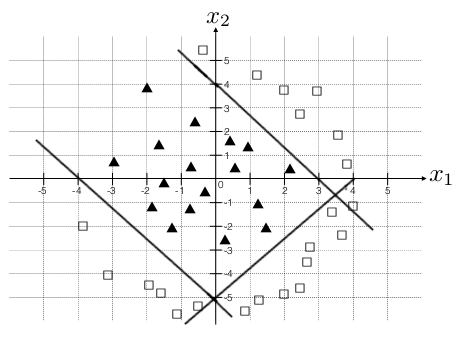
\includegraphics[width=50mm]{decisionregions.png}
	\end{center}
	\caption{Decision boundaries learned from the neural network}
\end{figure}

The topmost decision boundary is $-\frac{4}{3}x_1 - x_2 + 4 = 0$ For positive class membership it is necessary that $-\frac{4}{3}x_1 - x_2 + 4 > 0$. So $w_{11}=\frac{3}{4}$, $w_{21}=-1, b_1=4$ will give us that $h_j=1$ iff the necessary condition is satisfied. Likewise we have $\frac{5}{3}x_1 -x_2 -5 < 0$ which gives us $w_{12}=-\frac{5}{3}$, $w_{22}=1, b_2=5$. Finally, $-\frac{5}{4}x_1 -x_2 -5 < 0$ gives us $w_{13}=\frac{5}{4}$, $w_{23}=1, b_3=5$.
For membership in class 1, it easy to see that it is both neccessary and sufficient that $h_1 = h_2 = h_3 = 1$. If we set $u_1 = u_2 = u_3 = 1, c = -2.5$ we have that: 
$$f(x_1, x_2) = 1 \iff \sum_{j=1}^3 h_j - 2.5 > 0 \iff h_1 = h_2 = h_3 = 1$$
Giving us the desired result.

\section{Activation Functions}
\begin{enumerate}[(a)]
	\item We show that the derivative of the $ReLU(x) := \max(0,x)$ (where it exists) is the Heaviside step function:
	$$ H(x) = 
	\begin{cases} 
	1 & x > 0 \\
	0 & x < 0 \\ 
	\frac{1}{2} & x=0 
	\end{cases} \\
	$$
	We consider 3 cases. When $x>0$ we have that:
	\begin{align*}
	\dP{max(x,0)}{x}&=\lim\limits_{\epsilon\rightarrow0}\frac{\max(x+\epsilon,0)-\max(x,0)}{\epsilon} \\
	&=\lim\limits_{\epsilon\rightarrow0}\frac{x+\epsilon-x}{\epsilon}\\
	&= 1
	\end{align*}
	Where the second line follows when $x>|\epsilon|$. When x<0 we have:
	\begin{align*}
	\dP{max(x,0)}{x}&=\lim\limits_{\epsilon\rightarrow0}\frac{\max(x+\epsilon,0)-\max(x,0)}{\epsilon} \\
	&=\lim\limits_{\epsilon\rightarrow0}\frac{\max(x+\epsilon,0)}{\epsilon}\\
	&= 0
	\end{align*}
	Where, as before, the last line follows when $x>|\epsilon|$. When $x=0$ the limit does not exist. This is because the one sided limits are not equal:
		\begin{align*}
		\lim\limits_{\epsilon\rightarrow0^+}\frac{\max(\epsilon,0)}{\epsilon} &=\lim\limits_{\epsilon\rightarrow0^+}\frac{\epsilon}{\epsilon}= 1\\
		\lim\limits_{\epsilon\rightarrow0^-}\frac{\max(\epsilon,0)}{\epsilon} &= 0
		\end{align*}
	\item We can define $ReLU$ in terms of $H$ in the following way:
	\begin{align*}
	ReLU(x) &:= xH(x)\\
	ReLU(x) &:= \int_{t=-\infty}^{x} H(t)dt
	\end{align*} 
	\item We can write $H(x)$ as an asymptotic expression using $\sigma(x)$
	$$H(x) = 
	\lim\limits_{\epsilon \rightarrow\infty} \sigma(\epsilon x)
	$$
	\item As in (a) we break this into three pieces. Let $x>0$ then:
	\begin{align*} 
	\dP{H(x)}{x} &= \lim\limits_{\epsilon\rightarrow0}\frac{H(x+\epsilon)-H(x)}{\epsilon}\\
	&= \lim\limits_{\epsilon\rightarrow0}\frac{1-1}{\epsilon} \\
	&= 0
	\end{align*}
	Let $x<0$:
	\begin{align*} 
	\dP{H(x)}{x} &= \lim\limits_{\epsilon\rightarrow0}\frac{H(x+\epsilon)-H(x)}{\epsilon}\\
	&\lim\limits_{\epsilon\rightarrow0}\frac{0-0}{\epsilon} \\
	&= 0
	\end{align*}
	As in (a), the limit does not exist at $x=0$:
	\begin{align*}
	&\lim\limits_{\epsilon\rightarrow0^+}\frac{H(\epsilon)-\frac{1}{2}}{\epsilon} =\lim\limits_{\epsilon\rightarrow0^+}\frac{1-\frac{1}{2}}{\epsilon}=
	\lim\limits_{\epsilon\rightarrow0^+}\frac{1}{2\epsilon}= \infty
	\\
	&\lim\limits_{\epsilon\rightarrow0^-}\frac{H(\epsilon)-\frac{1}{2}}{\epsilon} = \lim\limits_{\epsilon\rightarrow0^-}\frac{0-\frac{1}{2}}{\epsilon} = \lim\limits_{\epsilon\rightarrow0^+}\frac{-1}{2\epsilon} = -\infty
	\end{align*}
	Notice $\dP{H(x)}{x} = 0$ for all $x \ne 0$ and that we can assign any value at $x=0$. If we let the derivative be $\infty$ at $0$ we have that $\dP{H(x)}{x}$ is the dirac delta function, as needed.
\end{enumerate}

\section{Gradients and Networks}
\begin{enumerate}[(a)]
	\item We compute the Jacobian of the softmax function $S(x)_i = \frac{\exp(x_i)}{\sum_k \exp(x_k)}$. First we consider the case where $i\ne j$
	\begin{align*}
	\dP{S(x)_i}{x_j} &= \dP{}{x_j}\frac{\exp(x_i)}{\sum_k \exp(x_k)}\\
	&=\exp(x_i)\dP{}{x_j}\left(\sum_k \exp(x_k)\right)^{-1}\\
	&=-\exp(x_i)\left(\sum_k \exp(x_k)\right)^{-2}\dP{}{x_j}\sum_k \exp(x_k)\\
	&=-\exp(x_i)\left(\sum_k \exp(x_k)\right)^{-2}\exp(x_j)\\
	&=-S(x)_iS(x)_j
	\end{align*}
	When $i=j$ we have that:
	\begin{align*}
	\dP{S(x)_i}{x_i} &= \frac{\exp(x_i)\left(\sum_k \exp(x_k)\right) - \exp(x_i)^2}{\left(\sum_k \exp(x_k)\right)^{2}}\\
	&= S(x)_i - \frac{\exp(x_i)^2}{\left(\sum_k \exp(x_k)\right)^{2}}\\
	&= S(x)_i - S(x)_i^2\\
	&= S(x)_i(1-S(x)_i)
	\end{align*}
	\item We can express (a) as the following matrix equation:
	$$ J(x) = Diag(S(x)) - S(x)S(x)^T$$
	Where $Diag(S(x))$ is a diagonal matrix whose $i^{th}$ entry is $S(x)_{i}$.
	\item We compute the jacobian matrix of the logistic sigmoid function, applied element-wise to $x$. For $i\ne j$ we have that:
	\begin{align*}
	\dP{\sigma(x)_i}{x_j} &= 0
	\end{align*}
	For $i=j$ we have:
	\begin{align*}
	\dP{\sigma(x)_j}{x_j} &= \dP{}{x_j}\frac{\exp(x_j)}{1 + \exp(x_j)}\\
	&= \frac{\exp(x_j)(1+\exp(x_j)) - \exp(x_j)^2}{(1 + \exp(x_j))^2}\\
	&= \frac{\exp(x_j)}{1+\exp(x_j)} - \left(\frac{\exp(x_j)}{1+\exp(x_j)}\right)^2\\
	&=\sigma(x_j)(1-\sigma(x_j))
	\end{align*}
	\item Let $y=f(x)$. From (c) we have $ J_y(x) = diag(\sigma'(x))$. Therefore, 
	\begin{align*}
	g_x &= diag(\sigma'(x))g_y \\
	&= \sigma'(x) \odot g_y
	\end{align*}
\end{enumerate}

\section{Softmax activation function}
\begin{enumerate}[(a)]
	\item We show the softmax is invariant under translation. Notice that:
	\begin{align*}
	S(x+c)_i &= \frac{\exp(x_i + c)}{\sum_k \exp(x_k + c)}\\
	&= \frac{\exp(c)\exp(x_i)}{\sum_k \exp(c)\exp(x_k)}\\
	&= \frac{\exp(x_i)}{\sum_k \exp(x_k)}\\
	&= S(x)_i
	\end{align*}
	\item If we multiply by a scalar greater than $1$, we increase the probability of the most probable classes. Likewise, if we multiply by a scalar less than $1$, we add probability to the less probable classes.
	
	\item We show that the two class softmax function can be written as the sigmoid function. Let $z = x_2 - x_1$, then:
	\begin{align*}
	\frac{1}{1+\exp(z)} &= \frac{1}{1 + \exp(x_2)\exp(-x_1)}\\
	&= \frac{\exp(x_1)}{\exp(x_1)+\exp(x_2)}\\
	\end{align*}
	And
	\begin{align*}
	1 - \frac{1}{1+\exp(z)} &= 1 - \frac{\exp(x_1)}{\exp(x_1)+\exp(x_2)}\\
	&= \frac{\exp(x_2)}{\exp(x_1)+\exp(x_2)}
	\end{align*}
	\item We express a $k$-class softmax as a function $f$ of $k-1$ variables. Define $z_i = x_i - x_1$ $\forall i \ne 1$. Then:
	\begin{align*}
	f(z_2, \cdots, z_{k})_i &= \begin{cases}
	\frac{\exp(z_i)}{\sum_{j=2}^{k} \exp(z_j) + 1} & i\ne 1\\
	1 - \sum_{j=2}^k f(z_{2},\cdots,z_{k})_j & i = 1
	\end{cases}
	\end{align*}
	We show that $f(z_2, \cdots, z_{k})_i = S(x_1, \cdots, c_k)_i$. For $i\ne 1$ we have that:
	\begin{align*}
	f(z_2, \cdots, z_{k})_i &= \frac{\exp(x_i-x_1)}{\sum_{j=2}^{k} \exp(x_j-x_1) + 1}\\
	&= \frac{\exp(x_i)}{\sum_{j=2}^{k} \exp(x_j) + \exp(x_1)}\\
	&= S(x_1, \cdots, c_k)_i
	\end{align*}
	For $i = 1$ the result follows since 
	$$S(x_1, \cdots, x_k)_1 = 1 - \sum_{j=2}^{k} S(x_1, \cdots, x_k)_j = 1 - \sum_{j=2}^k f(z_{2},\cdots,z_{k})_j$$

\end{enumerate}

\section{Using cross-entropy cost for real-valued data}
\begin{enumerate}[(a)]
	\item We derive the cross entropy cost function using the maximum likelihood principle. Let $X\in\{0,1\}$ and let $p = P(X=1)$
	\begin{align*}
	\log \mathcal{L}(p|x) &= \log p^x(1-p)^{1-x}\\
	&= x\log p + (1-x)\log(1-p)
	\end{align*}
	\item A probablistic interpreation of the cross entropy cost function would be the following. Denote the empirical density of $X$ as $\hat{p}(x)=x$ (that is, if $x=1$ then $p(X=0)=1$ and if $x=0$ then $p(X=1)=0$). Let $p(X=1)=p$ be our model distribution. Then, notice that:
	\begin{align*}
	KL(\hat{p},p) &= \sum_{x}\hat{p}(x)\log\frac{\hat{p}(x)}{p(x)}\\
	&= \sum_{x}\hat{p}(x)\log\hat{p}(x) - \sum_{x}\hat{p}(x)\log p(x)\\
	&= - \sum_{x}\hat{p}(x)\log p(x)
	\end{align*}
	Since $\hat{p}(x)\log\hat{p}(x) = 0$ since if $\hat{p}(x)=1$, $\log\hat{p}(x)=0$; and if $\hat{p}(x)=0$, $0\log 0 = 0$. We then have:
	\begin{align*}
	- \sum_{x}\hat{p}(x)\log p(x) = -x\log p -(1-x)\log(1-p)
	\end{align*}
	as needed.
\end{enumerate}

\newpage

\section{Deriving the Glorot initialization scheme}
\begin{enumerate}[(a)]
	\item We derive the Glorot initialization scheme from \cite{pmlr-v9-glorot10a}. We define $h_l$ as the hidden layer $l$ of size $d_l$, $a_l$ as a preactivation, $W_l$ as the incoming weights, $b_l$ as the bias term, and $g$ as the activation function. Additionally, we assume that for any neuron $i$ $h^i_{l}\sim \mathcal{N}(0,1)$. We have the following relations:
	\begin{align*}
	a_l &= b_l + \sum_{i=1}^{d_{l-1}} W_l^ih_{l-1}^i \\
	h_{l} &= g(a_l)
	\end{align*}
	We want to initialize $W_l$ and $b_l$ such that:
	\begin{enumerate}[(1)]
		\item $\Ex{}{a_l}=0$
		\item $\Var{a_l}=1$
	\end{enumerate}
	We notice that if we initialize $b_l$ as $0$ we can satisfy (1) since:
	\begin{align*}
	\Ex{}{a_l} &= \Ex{}{b_l} + \sum_{i=1}^{d_{l-1}} \Ex{}{W_l^i}\underbrace{\Ex{}{h_{l-1}^i}}_{=0}\\
	&= \Ex{}{b_l}
	\end{align*}
	To satisfy (2) we notice:
	\begin{align*}
	\Var{a_l}&= \Var{b_l + \sum_{i=1}^{d_{l-1}} W_l^ih_{l-1}^i}\\
	&= \sum_{i=1}^{d_{l-1}} \Var{W_l^i h_{l-1}^i }
	\end{align*}
	We drop the indices on $W_l$ and $h_{l-1}$ for clarity since each $h_{l-1}^i$ is iid, and we make the further assumption that $W_{l}^i$ is initialized such that it is iid. We get that:
	\begin{align*}
	\Var{a_l} &= d_{l-1} \Var{W_lh_{l-1}}\\
	&=d_{l-1} \Ex{}{W_l^2}\Ex{}{h_{l-1}^2} - d_{l-1} \Ex{}{W_l}^2\underbrace{\Ex{}{h_{l-1}}^2}_{=0}\\
	&= d_{l-1} \Var{W_l}\Ex{}{h_{l-1}^2}
	\end{align*}
	Since $h_{l-1}\sim\mathcal{N}(0,1)$, we have that $\Ex{}{h_{l-1}^2} = \Var{h_{l-1}} + \Ex{}{h_{l-1}}^2 = 1$. Putting this together gives us:
	\begin{align*}
	\Var{a_l} &= d_{l-1} \Var{W_l}
	\end{align*}
	With $L$ layers we have that:
	\begin{align*}
	\Var{a_L} &= \Var{ a_1} \prod_{k=2}^{L} d_{k-1} \Var{W_k}
	\end{align*}
	In order to satisfy (2) we must initialize each $W_l$ such that $\forall k \ d_{k-1}\Var{W_k} = 1$, provided each $W_l$ is iid and are independent of each $h_l$\footnote{recall that we dropped the indices}. One way of doing this is to initialize each $b_l=0$, $W_1\sim\mathcal{N}(0,1)$, and for each subsequent layer, $W_l\sim\mathcal{N}\left(0,\frac{1}{d_{l-1}}\right)$.
	
	\item We maintain all the assumptions from (a) except $h_l$ is no longer Normally distributed and instead, $a_l$ is Normally distributed. We also assume that:
	\begin{align*}
	h_l = g(a_l) = \max\{0, a_l\}
	\end{align*}
	We notice that even if we initialize $b_l$ as $0$, we won't satisfy (1) since $\Ex{}{h_l}$ is no longer necessarily $0$. We overcome this by initializing $W_l$ such that its mean is $0$. To satisfy (2) we notice:
	\begin{align*}
	\Var{a_l} &=d_{l-1} \Ex{}{W_l^2}\Ex{}{h_{l-1}^2} - d_{l-1} \underbrace{\Ex{}{W_l}^2}_{=0}\Ex{}{h_{l-1}}^2\\
	&= d_{l-1} \Var{W_l}\Ex{}{h_{l-1}^2}
	\end{align*}
	We can compute the second moment of $h_{l-1}$ easily since the Normal distribution is symmetric and $\Ex{}{a_{l-1}}=0$:
	\begin{align*}
	\Ex{}{h_{l-1}^2} &= \int_{-\infty}^{\infty} \max\left\{ 0, a_{l-1} \right\}^2 p(a_{l-1})da_{l-1}\\
	&= \int_{0}^{\infty} a_{l-1}^2 p(a_{l-1})da_{l-1}\\
	&=\frac{1}{2}\Ex{}{a_{l-1}^2}\\
	&= \frac{1}{2} \Var{a_{l-1}}
	\end{align*}
	As with (a), if we substitute this into the previous expression we get: 
	\begin{align*}
	\Var{a_l} &= \frac{d_{l-1}}{2} \Var{W_l}\Var{ a_{l-1}} \\
	\Var{a_L} &= \Var{ a_1} \prod_{k=2}^{L} \frac{d_{k-1}}{2} \Var{W_k}
	\end{align*}
	And so, using the same reasoning as in (a), we can satisfy (1) and (2) by initializing each $b_l=0$, $W_1\sim\mathcal{N}(0,1)$, and for each subsequent layer, $W_l\sim\mathcal{N}\left(0,\frac{2}{d_{l-1}}\right)$.
\end{enumerate}

%We derive the Glorot initialization scheme from \cite{pmlr-v9-glorot10a} for a ReLU layer using the approach from \cite{He:2015:DDR:2919332.2919814} . As defined in the notes, let:
%\begin{align*}
%a^{(k)}(x)_i &= b_i^{(k)} + \sum_{j=1}^n w_{ij}^{(k)}h^{(k-1)}(x)_j \\
%h^{(k)}(x)_j &= g(a^{(k)}(x)_j)\\
%&= \max\left\{ 0, a^{(k)}(x)_j \right\}
%\end{align*}
%We suppose that each $w_{ij}^{(k)}$ is sampled iid from a zero mean symmetric distribution, and that each $h^{(k-1)}(x)_j$ is sampled iid from an independent symmetric distribution. We have that:
%\begin{align*}
%Var\left\{a^{(k)}(x)_i\right\}&= Var\left\{\sum_{j=1}^{n_k} w_{ij}^{(k)}h^{(k-1)}(x)_j\right\}\\
%&= n_k Var\left\{w^{(k)}h^{(k-1)}\right\}\\
%&= n_k \Ex{}{(w^{(k)})^2}\Ex{}{(h^{(k-1)})^2} - n \underbrace{\Ex{}{w^{(k)}}^2}_{=0}\Ex{}{h^{(k-1)}}^2\\
%&= n_k Var\left\{w^{(k)}\right\}\Ex{}{(h^{(k-1)})^2}
%\end{align*}
%Note that we drop the subscripts from both $w$ and $h$ and the argument from $h$ for clarity. If $w^{(k-1)}$ has a symmetric distribution around 0 and that each $b^{(k-1)}=0$ then $a^{(k-1)}$ is symmetric about 0 and has 0 mean. We have that:
%\begin{align*}
%\Ex{}{(h^{(k-1)})^2} &= \int_{-\infty}^{\infty} \max\left\{ 0, a^{(k-1)} \right\}^2 p(a^{(k-1)})da^{(k-1)}\\
%&= \int_{0}^{\infty} (a^{(k-1)})^2p(a^{(k-1)})da^{(k-1)}\\
%&=\frac{1}{2}\Ex{}{(a^{(k-1)})^2}\\
%&= \frac{1}{2} Var\left\{ a^{(k-1)}\right\}
%\end{align*}
%Substituting this into the previous expression yields:
%\begin{align*}
%Var\left\{a^{(k)}(x)_i\right\} &= \frac{n_k}{2} Var\left\{w^{(k)}\right\}Var\left\{ a^{(k-1)}(x)_i\right\}
%\end{align*}
%With $L$ layers we have that:
%\begin{align*}
%Var\left\{a^{(L)}(x)_i\right\} &= Var\left\{ a^{(1)}(x)_i\right\} \prod_{k=1}^{L} \frac{n_k}{2} Var\left\{w^{(k)}\right\}
%\end{align*}
%We see that in order to keep the variances consistent between levels it is enough to have $\frac{n_k}{2} Var\left\{w^{(k)}\right\} = 1$ $\forall k$. One way to satisfy this along with the assumptions above is to initialize each $w^{(k)}$ from a $\mathcal{N}\left(0, \sqrt{\frac{2}{n_k}}\right)$ and initialize each $b^{(k)}=0$.
%
%
%For the backwards case, we use that:
%\begin{align*}
%\dP{Cost}{h^{(k-1)}(x)_j} &= \sum_{i=1}^m w_{ij}^{(k)} \dP{Cost}{a^{(k)}(x)_i}\\
%\dP{Cost}{a^{(k)}(x)_i} &= g'(a^{(k)}(x))_i\dP{Cost}{h^{(k)}(x)_i}
%\end{align*}
%We assume that each $w_{ij}^{(k)}$ and $\dP{Cost}{a^{(k)}(x)_i}$ are mutually independent, and each $w_{ij}^{(k)}$ comes from a distribution symmetric around 0 with 0 mean. This implies that $\dP{Cost}{h^{(k-1)}(x)}$ has 0 mean since:
%\begin{align*}
%\Ex{}{\dP{Cost}{h^{(k-1)}(x)_i}}&=\Ex{}{\sum_{i=1}^m w_{ij}^{(k)} \dP{Cost}{a^{(k)}(x)_i}}\\
%&= \sum_{i=1}^m\underbrace{\Ex{}{ w_{ij}^{(k)} }}_{=0} \Ex{}{\dP{Cost}{a^{(k)}(x)}} \\
%&= 0
%\end{align*}
%We assume that $g'(a^{(k)})$ and $\dP{Cost}{h^{(k)}}$ are independent (dropping the subscripts and arguments once more) to get:
%\begin{align*}
%\Ex{}{\dP{Cost}{a^{(k)}}} &= \Ex{}{g'(a^{(k)})}\Ex{}{\dP{Cost}{h^{(k)}}}\\
%&\overset{(a)}{=} \frac{1}{2}\Ex{}{\dP{Cost}{h^{(k)}}} \\
%&\overset{(b)}{=} 0
%\end{align*}
%Where (a) follows since $g'(a^{(k)})=H(a^{(k)}) = 1$ wp $\frac{1}{2}$ and is $0$ otherwise, and (b) follows from the previous claim. We then get:
%\begin{align*}
%Var\left\{\dP{Cost}{a^{(k)}}\right\} &=\Ex{}{\left(\dP{Cost}{a^{(k)}}\right)^2} \\
%&=\int_{-\infty}^{\infty} \left(H(a^{(k)}) \dP{Cost}{h^{(k)}}\right)^2 p(a^{(k)})da^{(k)}\\
%&=\int_{0}^{\infty} \dP{Cost}{h^{(k)}}^2p(a^{(k)})da^{(k)}\\
%&= \frac{1}{2}Var\left\{\dP{Cost}{h^{(k)}}\right\}
%\end{align*}
%We compute the variance as before: 
%\begin{align*}
%Var\left\{\dP{Cost}{h^{(k-1)}}\right\} &= \frac{m_k}{2} Var\left\{w^{(k)}\right\} Var\left\{\dP{Cost}{h^{(k)}}\right\}
%\end{align*}
%With $L$ layers we have that:
%\begin{align*}
%Var\left\{\dP{Cost}{h^{(2)}}\right\} &= Var\left\{\dP{Cost}{h^{(L+1)}}\right\} \prod_{k=1}^{L} \frac{m_k}{2} Var\left\{w^{(k)}\right\}
%\end{align*}
%Using identical reasoning as with the forward case, it is enough to initialize each $w^{(k)}$ from a $\mathcal{N}\left(0, \sqrt{\frac{2}{m_k}}\right)$ and initialize each $b^{(k)}=0$.
\newpage

\bibliographystyle{ieeetr}
\bibliography{A1.bib}


\end{document}